%%%%%%%%%%%%%%%%%%%%%%%%%%%%%
% Folkeskolens afgangsprøve %
%%%%%%%%%%%%%%%%%%%%%%%%%%%%%

\documentclass[a4,12pt]{article}

% Danish character input and hyphenations.
\usepackage[danish]{babel}
\usepackage[utf8]{inputenc}

% Gives hyperlinks in PDF file.
\usepackage[colorlinks=true, linkcolor=blue]{hyperref}

% AMS math package for nice equation and math options.
\usepackage{amsmath}
% Restart numbering for each section and prefix with section number.
\numberwithin{equation}{section}
\numberwithin{table}{section}
\numberwithin{figure}{section}

% Set margins.
\usepackage[top=3cm, bottom=3cm, left=2cm, right=2cm]{geometry}

% Handle raster and vector graphics (e.g. PNG, EPS and PDF).
\usepackage{graphicx}

% Nice tabular (tables) environment.
\usepackage{tabularx}

% Maybe this will come in handy in the future.
\usepackage{tabu}

% For being able to reference the page number of the last page.
\usepackage{lastpage}

% Page breaks before all sections.
\usepackage{titlesec}
\newcommand{\sectionbreak}{\clearpage}

%%%%%%%%%%%%%%%%%%%%%
% Husk at udfylde!! %
%%%%%%%%%%%%%%%%%%%%%
\newcommand{\skoleklasse}{8.D} % <=== Ret til eksamen.
\newcommand{\proevetype}{Folkeskolens afgangsprøve}
\newcommand{\proevefag}{Matematik}
\newcommand{\elevnavn}{Sofus Dawids}
\newcommand{\elevnummer}{N/A} % <=== Ret til eksamen.
\newcommand{\tilsynshavende}{SP} % <=== Ret til eksamen.
\newcommand{\eksamensdato}{xx. måned 201X} % <=== Ret til eksamen.
\newcommand{\antalarkialt}{\pageref*{LastPage} \textbf{Kontroller!}} % <=== Kontroller til eksamen.

% Front page box for exam.
\newcommand{\eksamensforsideboks}{
\noindent
\begin{tabu} to  \textwidth {|X[c]|}
  \hline
  \tabulinesep=^1pt
  \begin{tabu} {@{}X[1,l]X[3,c]X[1,r]@{}}
    Skolenr. 173004 & {\large \textbf{HUMMELTOFTESKOLEN}} & Tlf: 4585 4649 \\
  & 2830 Virum & \\
  \end{tabu} \\
  \hline
  \begin{tabu} {@{}lX[l]|ll@{}}
    Prøve: & \proevetype & Dato: & \eksamensdato \\
    Fag: & \proevefag & Klasse: & \skoleklasse \\
    Elevens navn: & \elevnavn & Elevnr.: & \elevnummer \\
    Elevunderskrift: & & Antal ark i alt: & \antalarkialt \\[0.5cm]
  \end{tabu} \\
  \hline
  \begin{tabu} {@{}l|lX[l]|ll@{}}
    Tilsynshavende & Underskrift: & & Initialer: & \tilsynshavende \\[0.5cm]
  \end{tabu} \\
  \hline
\end{tabu}
\vspace{1cm}
}

% Headers and footers.
\usepackage{fancyhdr}
\pagestyle{fancy}
\newcommand{\eksamensfooter}{%
  \lfoot{\elevnavn \\ Hummeltofteskolen \skoleklasse}
  \cfoot{\eksamensdato \\ side~\thepage~af~\pageref*{LastPage}}
  \rfoot{\proevefag \\ Elevnummer \elevnummer}
  \renewcommand{\footrulewidth}{0.4pt}
}
\eksamensfooter
\fancypagestyle{plain}{%
  \fancyhf{}
  \renewcommand{\headrulewidth}{0.0pt}
  \eksamensfooter
}

\makeatletter
\newcommand*{\tableofcontentsnobreak}{\@starttoc{toc}}
\makeatother

% End of preamble and beginning of text.
\begin{document}

\thispagestyle{plain}
\eksamensforsideboks

\tableofcontentsnobreak

\section{Første opgave}
Start første opgave her\ldots

Brug \verb$\section{...}$ for hvert ny opgave.

% Bilag starter herefter.
\appendix
\section{Første bilagsafsnit}
Start første \emph{bilagsafsnit} her\ldots

Brug \verb$\section{...}$ for hvert nyt bilagsafsnit.

\section{Eksempler -- slettes før aflevering}
Her er en række brugbare eksempler.

\subsection{Formler i teksten}
For at lave en formel midt i den løbende tekst, skriver man \verb$\($ og \verb$\)$ omkring formlen.
Så kommer det til at se således ud med \( a^2 + b^2 = c^2 \) midt i teksten.

\subsection{Fritstående formler}
For at lave en formel som står for sig selv, bruger man \verb$\[$ og \verb$\]$ ovenfor og nedenfor formlen på linjer for sig selv således:
\[
  \sum\limits_{n=1}^\infty{\pi \over n^2}
    = \pi \cdot \sum\limits_{n=1}^\infty{1 \over n^2}
    = 2\pi
\]
For at få nummereret formlen, benytter man \verb$equation$ environment:
\begin{equation}
  \sum\limits_{n=1}^\infty{\pi \over n^2}
    = \pi \cdot \sum\limits_{n=1}^\infty{1 \over n^2}
    = 2\pi
\end{equation}


\subsection{Henvisninger}
For at henvise til en ting -- fx en formel, så sætter man en \verb$\label$ i objektet og benytter \verb$\ref$ og \verb$\pageref$ til at henvise. Her er en formel
\begin{equation}
  a^2 + b^2 = c^2
  \label{eq:pytagoras}
\end{equation}
Her henviser vi så til formlen, som har nummer~\ref{eq:pytagoras} og står på side~\pageref{eq:pytagoras}. Bemærk, at der er indsat \verb$~$ mellem tekst og reference. Det er et \emph{non-breaking space}, så vi undgår et linjeskift her. Husk at køre \verb$pdflatex$ to gange for at opdatere referencer.

\subsection{Tabeller}
For at lave en tabel, bruger man \verb$tabular$, \verb$tabularx$ eller \verb$tabu$ environment.

Her er en simpel tabel:

\noindent
\begin{tabu}{|l|c|r|}
  \hline % vandret linje _over_ denne række.
  \rowfont{\bfseries} % Denne række er i fed.
  venstrestillet & centreret & højrestillet \\ % Linjeskift
  \hline % vandret linje _over_ denne række.
  l & c & r \\
  \hline % vandret linje nederst
\end{tabu}

Her er en anden tabel, hvor midterste kolonne strækker sig. Derfor har vi angivet bredden til hele siden. Man kunne også angive en eksakt bredde, fx 5cm.

\noindent
\begin{tabu} to \textwidth {|l|X[c]|r|}
  \hline % vandret linje _over_ denne række.
  \rowfont{\bfseries} % Denne række er i fed.
  venstrestillet & centreret & højrestillet \\
  \hline % vandret linje _over_ denne række.
  l & c & r \\
  \hline % vandret linje nederst
\end{tabu}

\subsection{Placering}
Man bør ikke placere tabeller og figurer midt i teksten, da det ikke er sikkert, at de kan være lige der. Derfor skal man overlade beslutningen til \LaTeX, så de placeres bedst muligt. Til det formål benytter man \verb$table$ og \verb$figure$ environments. Så får man også nummereret tabeller og figurer.

\begin{table}[htp] % Placer her (h), på toppen af samme side (t) eller på egen side (p).
  \centering
  \begin{tabu}{|l|c|r|}
    \hline % vandret linje _over_ denne række.
    \rowfont{\bfseries} % Denne række er i fed.
    venstrestillet & centreret & højrestillet \\ % Linjeskift
    \hline % vandret linje _over_ denne række.
    l & c & r \\
    \hline % vandret linje nederst
  \end{tabu}
  \caption{En simpel tabel}
  \label{table:simpel}
\end{table}

Se fx tabel~\ref{table:simpel}, som automatisk er placeret på side~\pageref{table:simpel}.

\subsection{Tegninger og billeder}
Man kan inkludere billeder i forskellige grafikformater. Foretræk vektorgrafik som fx PDF (eller EPS). Ellers kan man bruge PNG (tabsfrit) eller JPG.

Her er to figurer i henholdsvis PNG i kun 72 dpi (figur~\ref{figure:enhedscirklenpng72}) og i PDF (figur~\ref{figure:enhedscirklenpdf}).

\begin{figure}[htp]
  \centering
  
\includegraphics[width=5cm]{Enhedscirklen72.png}
  \caption{Enhedscirklen i PNG (72dpi)}
  \label{figure:enhedscirklenpng72}
\end{figure}

\begin{figure}[htp]
  \centering
  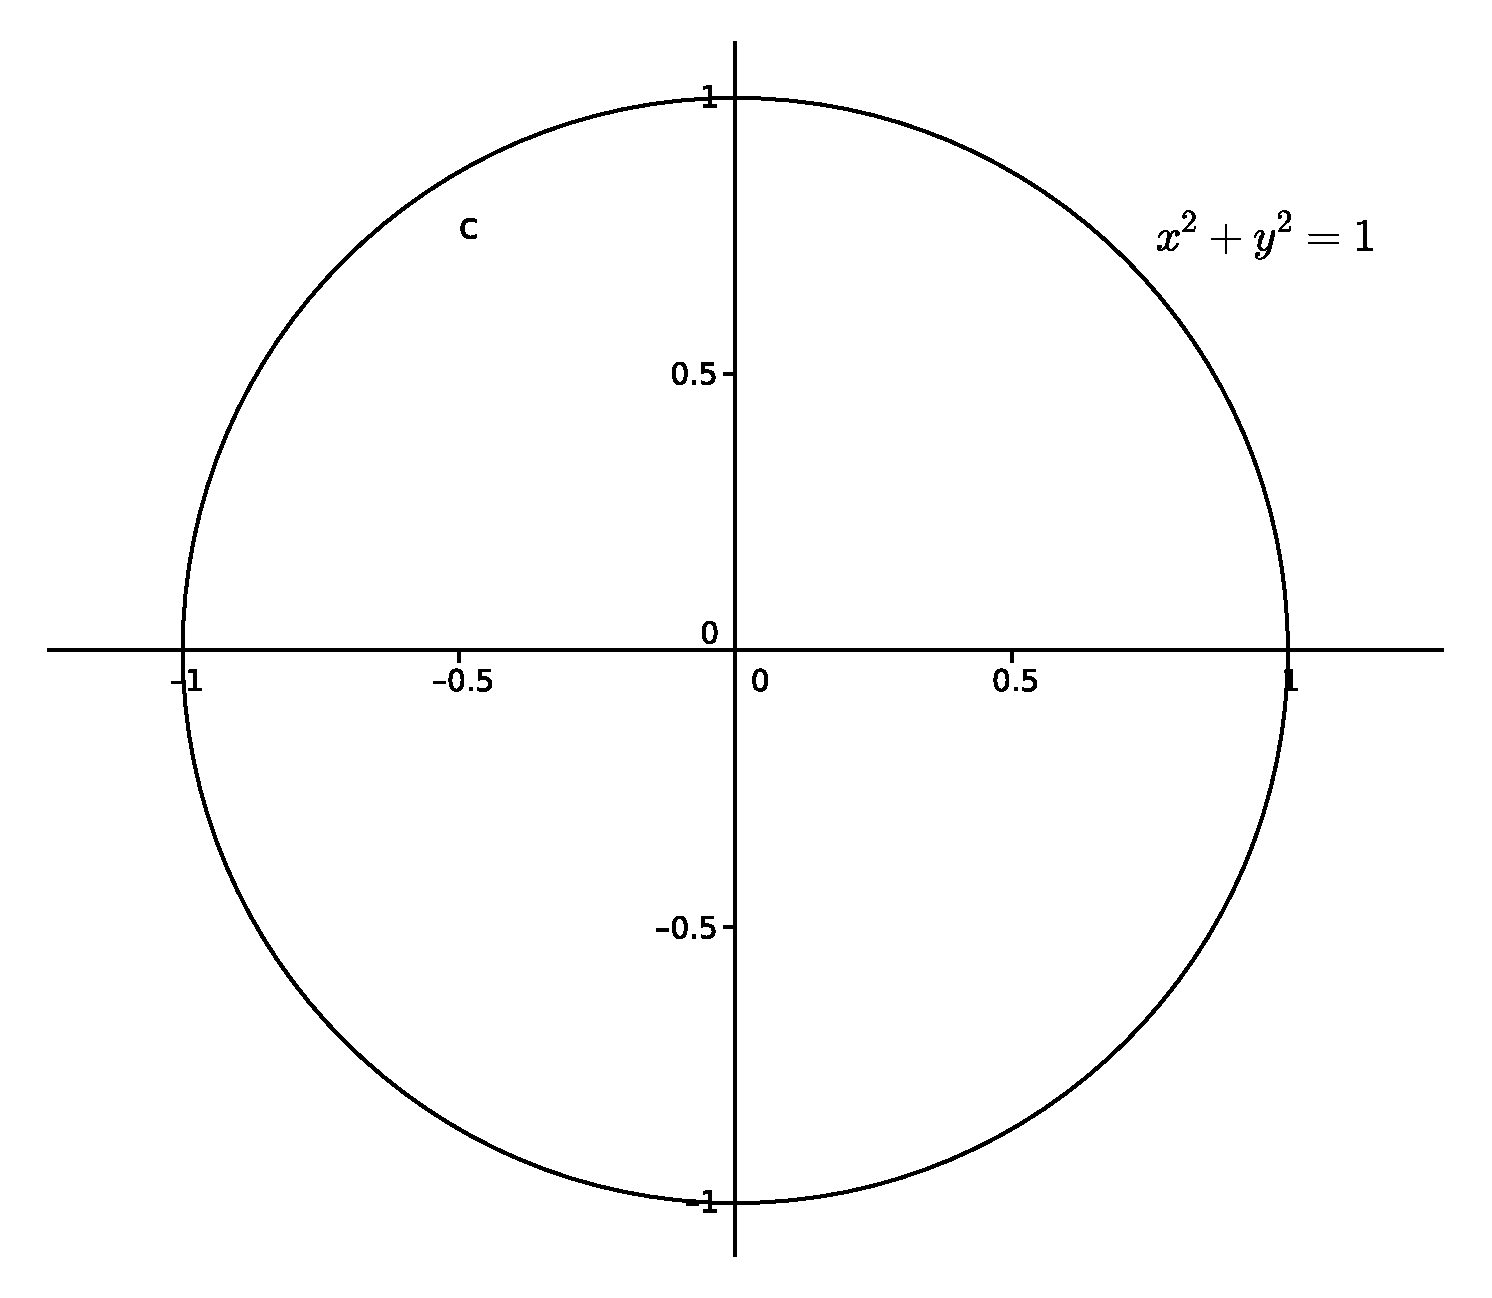
\includegraphics[width=5cm]{Enhedscirklen.pdf}
  \caption{Enhedscirklen i PDF}
  \label{figure:enhedscirklenpdf}
\end{figure}

% End of document.
\end{document}

